Figure \ref{fig:Clean} represents a MRI of a patient with brain tumour. Figure \ref{fig:CleanGray} shows the area of pathological tissue.

\begin{figure}
\centering
    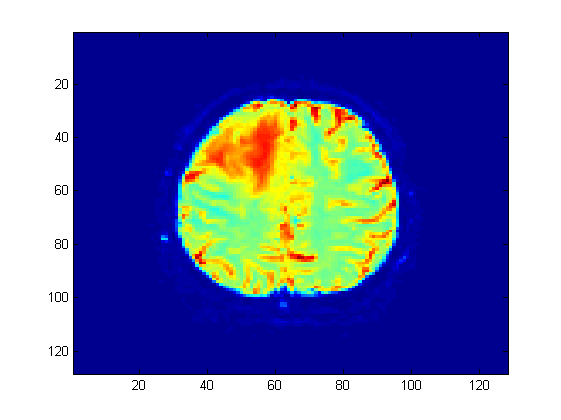
\includegraphics[scale=0.5,angle=0]{Imageclean.png}
    \caption{First image of the MRI with false color.}
    \label{fig:Clean}
\end{figure}

\begin{figure}
\centering
    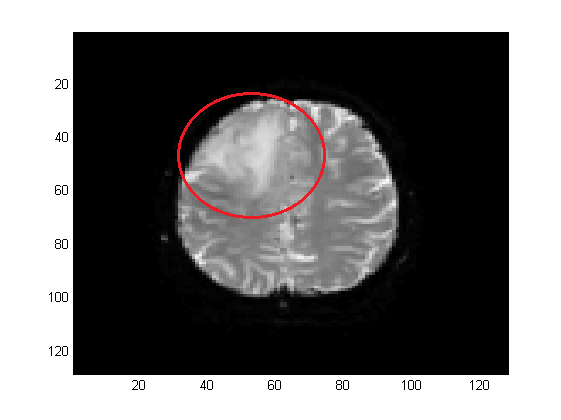
\includegraphics[scale=0.5,angle=0]{ImageGray.png}
    \caption{Area presenting the pathology.}
    \label{fig:CleanGray}
\end{figure}

By applying Algorithm \ref{alg:algorithm1} on the ROI with a number of class $N_{class} = 2$ and $N_{class} = 3$, we get some results which are shown in Figures \ref{fig:Result},\ref{fig:Result2},\ref{fig:Result3}.

\begin{figure}
\centering
    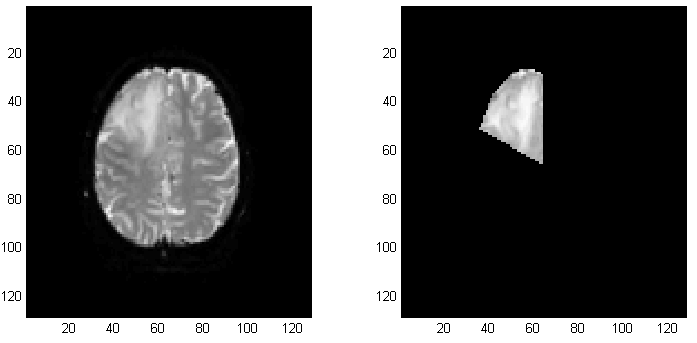
\includegraphics[scale=0.45,angle=0]{Result.png}
    \caption{Results of the algorithm. left: MRI image. right: Mask applied.}
    \label{fig:Result}
\end{figure}

\begin{figure}
\centering
    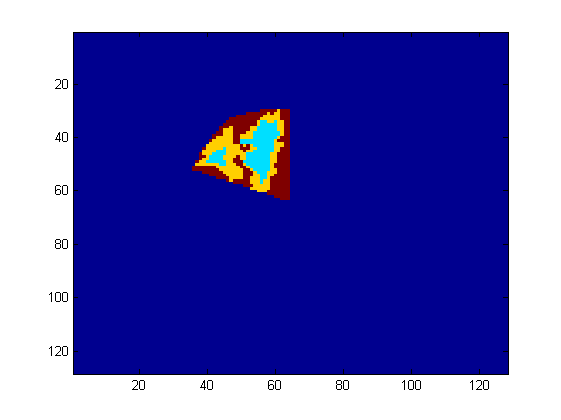
\includegraphics[scale=0.5,angle=0]{3class.png}
    \caption{The results of the algorithm for $N_{class} = 2$.}
    \label{fig:Result2}
\end{figure}

\begin{figure}
\centering
    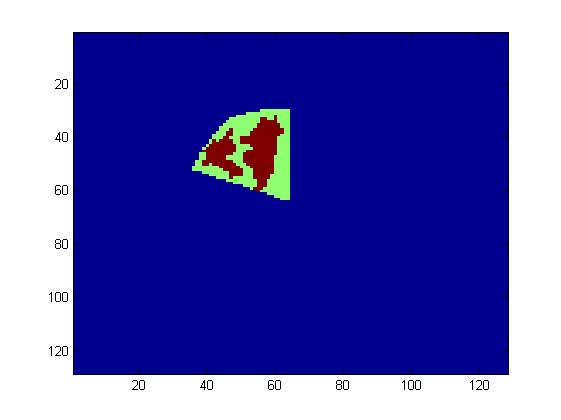
\includegraphics[scale=0.5,angle=0]{2class.png}
    \caption{The results of the algorithm for $N_{class} = 2$.}
    \label{fig:Result3}
\end{figure}

Our experimental results show that the algorithm can easily isolate the pathology from the normal tissues. By adjusting $N_{class} = 3$, we can generate a third class representing the uncertain zone.

\medskip

The results are satisfying. Our similitude matrix depends only on the neighbourhood of each point so our processing tool-chain is highly independent of the input data. Furthermore, the process is fully automated. The user must provide only the number of class and our program deal with the data in order to calculate the truth table.

Nevertheless, when we are trying to apply other algorithms in order to automatically find the optimal number of class \cite{zelnik2004self}, \cite{mouysset2010contributions}, the results aren't satisfying in the case of real data. For now, our only choice is to provide a set of maps with different value of $N_{class}$ and interpret the results, as it has been done with Figure \ref{fig:Result}, \ref{fig:Result2}, \ref{fig:Result3}.

\medskip

The processing tool-chain that have been implemented have been realized in order to have in the end the exact number of cluster $N$ when we apply the k-means algorithm. That means that in some case the algorithm wouldn't arrive to this number of class but we don't allow this situation to happen. It may have a huge impact on the algorithm.